\documentclass[a4paper]{article}
\usepackage{graphicx}
\usepackage{blindtext}
\usepackage{watermark}
\usepackage[ngerman]{babel}
\usepackage{caption, booktabs}
\usepackage{ltxtable}
\usepackage{float}
\selectlanguage{german}
%\selectlanguage{english}


\thiswatermark{\put(-129,-748){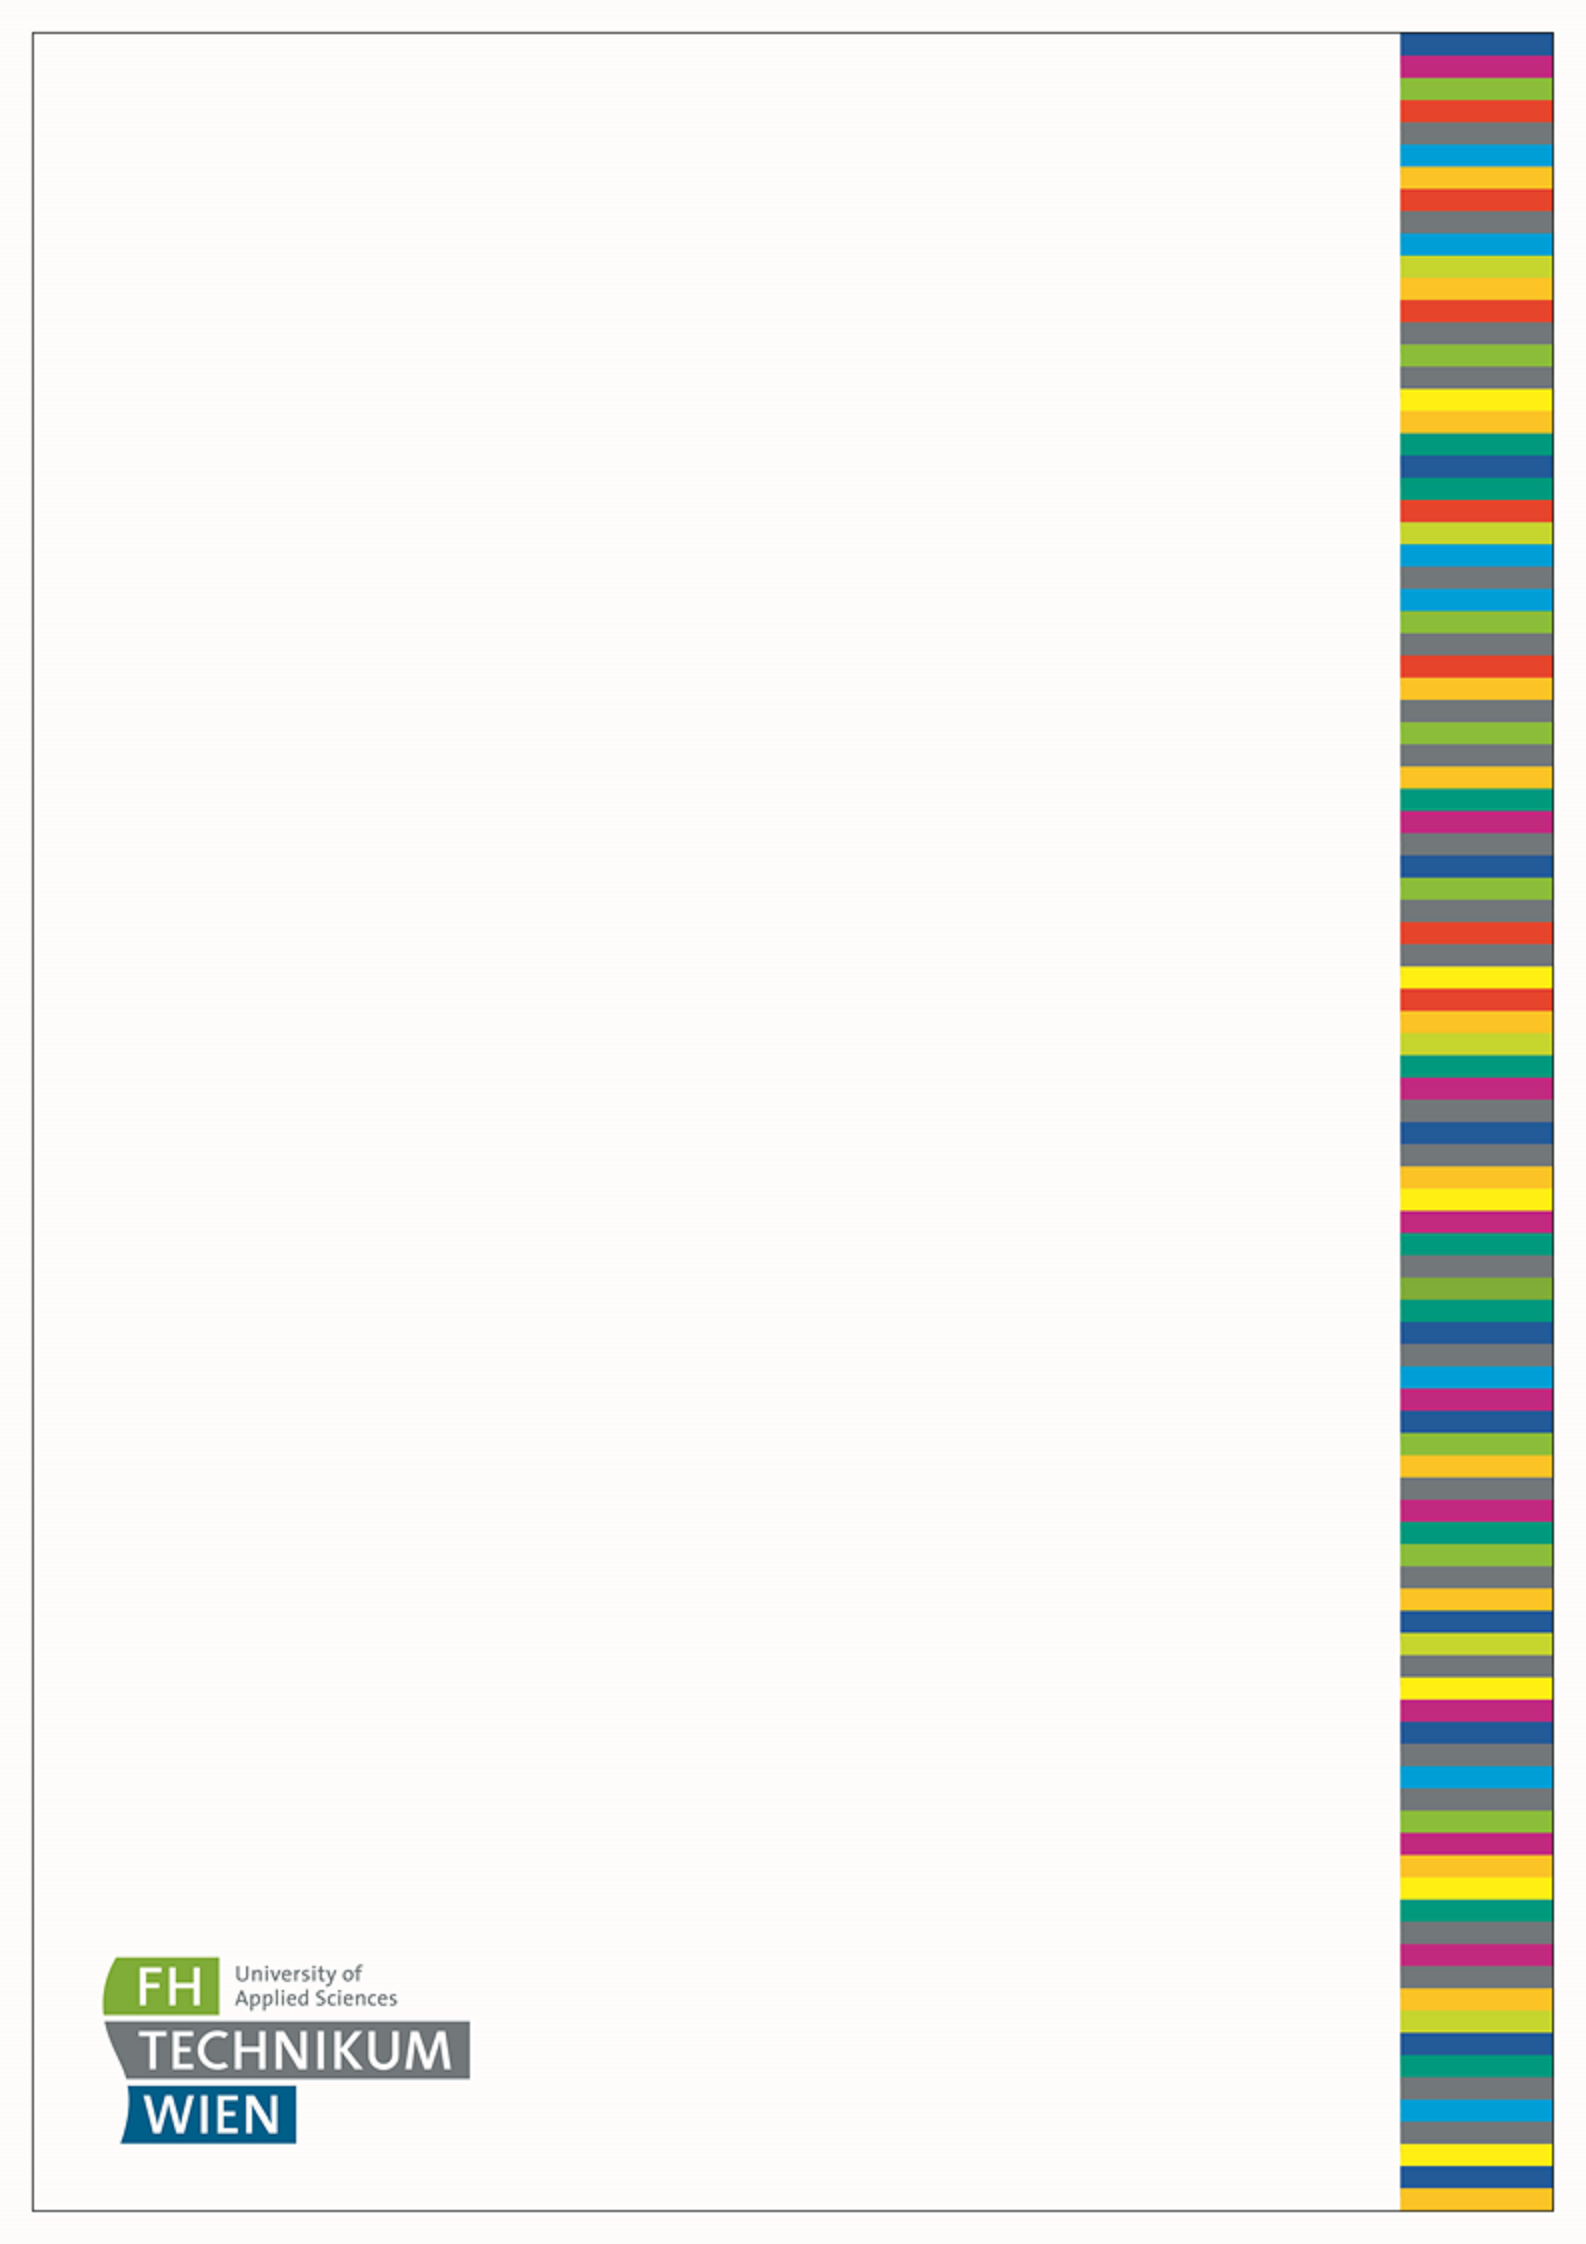
\includegraphics[scale=0.506]{Image/Titelblatt.png}}}

\title{{\huge Übung 2}\\Laborsimulationsprotokoll\\ \large im Studiengang Mechatronik/Robotik (Bachelor) Lehrveranstaltung IC-Übung}
\date{Begutachter: Dr. Moritz Lang \\ WS2020}
\author{Caspar J.F. Conradi (mr19b041) \and Tobias Grill (mr19b026)}





\begin{document}

    \maketitle
    \pagenumbering{gobble}
    \newpage
    \pagenumbering{arabic}


    %titelblatt & Diskussion -> Caspar
    %Spielelogik, Schaltplan, Funktionen -> Grill

    
    \begin{figure}[h!] %das [h!] macht das das Foto auch wkl an der richtigen Stelle ist
		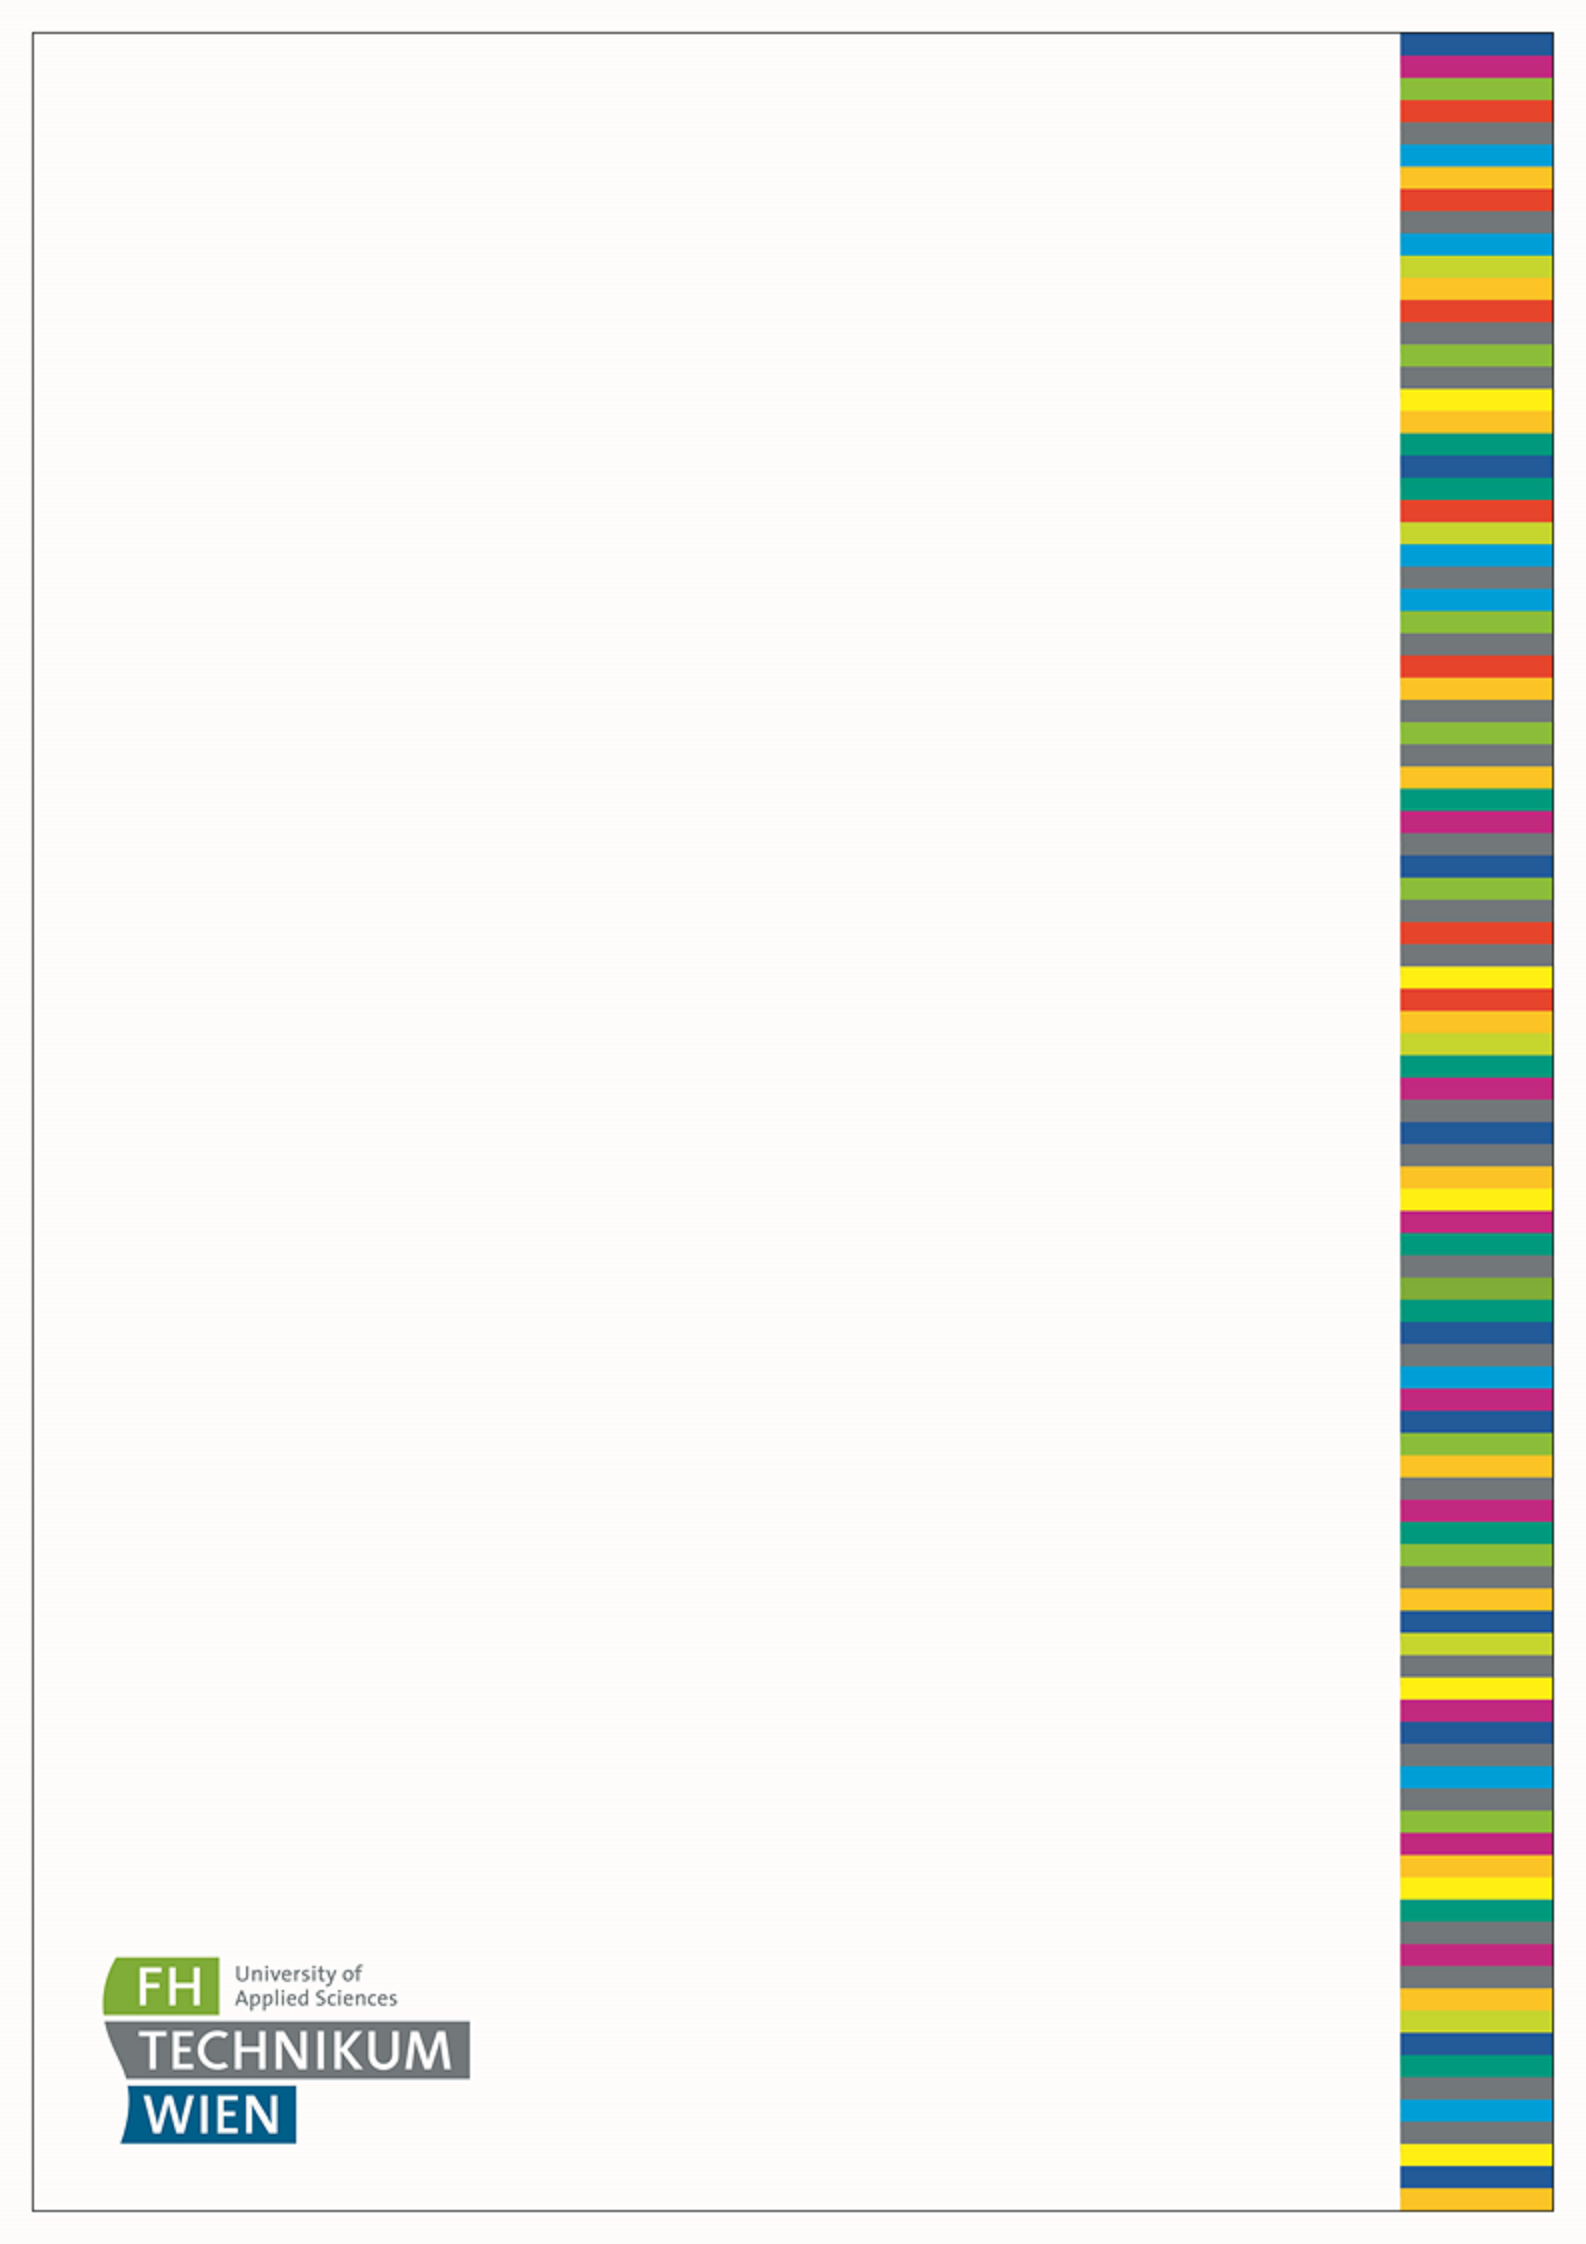
\includegraphics[width=\linewidth]{Image/Titelblatt.png}
	\end{figure}

    
    %titelblatt & Diskussion -> Caspar
    %Spielelogik, Schaltplan, Funktionen -> Grilli


    \newpage
    \tableofcontents
    \newpage

    %\titelblatt??????????????
    \section{Spielelogik}
     In dieser Übung wird das Spiel "Pong" programmiert. Das Spielfeld wird mit acht LEDs simuliert, die Anzahl der LEDs kann allerdings aufgrund der dynamischen programmierung schnell verändert werden, ohne dass sich die Spiellogik bzw. die Funktion ändert. Die Position des Balles wird durch aufleuchten der entsprechenden LED angezeigt. Wobei die LED ganz links den Annahmebereich des linken Spielers entspricht und die LED ganz rechts den Annahmebereich des rechten Spielers.\\
     Das Spiel ist so aufgebaut, dass zwei Spieler gegeneinander Spielen können. Durch betätigen des Tasters S1, wird der Ball vom linken Spieler zurückgeschlagen und durch drücken des Tasters S2 vom rechten Spieler zurückgeschlagen. Wird ein Taster fälschlicherweise betätigt, also wenn sich der Ball nicht im entsprechenden Annahmebereich befindet, hat der Spieler die Runde verloren. Wird der Ball nicht korrekt angenommen, sollen die LEDs fünf Sekunden lang in einer bestimmten Sequenz aufleuchten und der Spieler der verloren hat, bekommt den Ball. Ein neues Spiel wird erst nach einem Aufschlag gestartet.\\
     Außerdem wird die Schwierigkeit erhöht, indem der Ball kontinuierlich beschleunigt. Die Geschwindigkeit des Balles verdoppelt sich alle fünf Sekunden. Bei Spielstart wird die Geschwindigkeit wider auf die Anfangsgeschwindigkeit gesetzt.

     \subsection{Spielparameter}
      Die folgenden Parameter bestimmen zu einen großen Teil den Spielablauf. Falls man einen Wert davon ändern möchte, reicht es diesen in der Datenstruktur typePongConfigurations bzw. typePongState anzupassen, ohne weiteren Code zu ändern.
     \begin{table}[h!]
       \begin{center}
         \begin{tabular}{|l|c|r|}
        \hline 
           \textbf{Variable} & \textbf{Initialwert} & \textbf{Beschreibung}\\
           \hline
           fieldWidth & 23,77 & Bestimmt die größe des Spielfeldes\\
           \hline
           kickBackArea & 2,971 & Bestimmt die größe des Annahmebereichs\\
           \hline
           ballSpeed & 4 & Bestimmt die Ballgeschwindigkeit\\
           \hline
           lampNmbr[  ] & 7 & Anzahl der LEDs\\
           \hline
         \end{tabular}
         \caption{Spielparameter}
         \label{tab:Spielparameter}
       \end{center}
     \end{table}

    \section{Schaltplan}    %Screenshots von MatLab und beschreiben?
    
     \begin{figure}[H]
         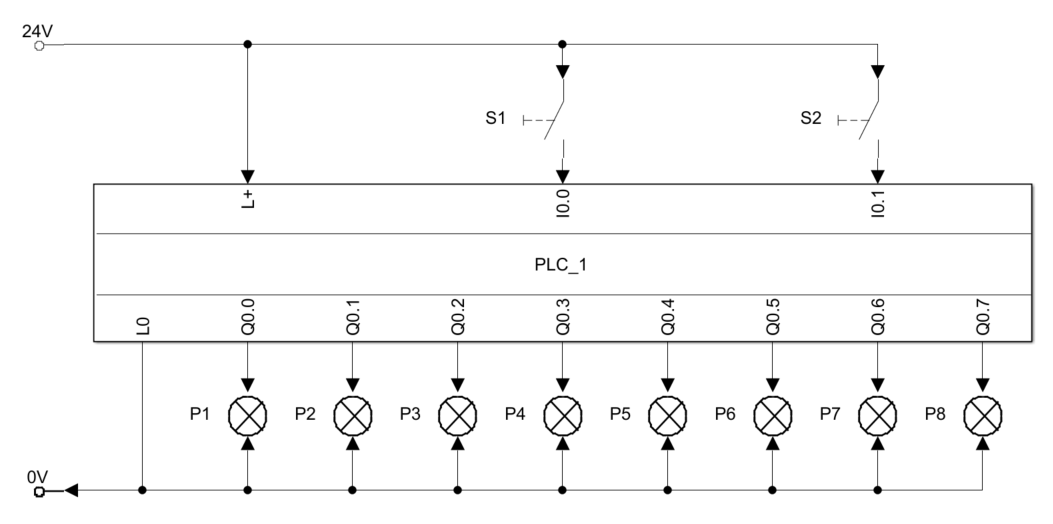
\includegraphics[width=\linewidth]{Image/Schaltplan.PNG}
         \caption{Schaltplan aus MatLab}
     \end{figure}

     Wird der Taster S1 betätigt, und somit ein Signal am Eingang I0.0 gelegt, wird der Ball vom linken Spieler angenommen. Analog dazu ist der Taster S2 am Eingang I0.1 für den rechten Spieler.\\
     Die LEDs P1 - 8, an den Ausgängen Q0.0 - 0.7, zeigen die Position des Balles an. Die Anzahl kann beliebig erhöht od verringert werden, vorrausgesetzt die entsprechende Variable, wie in Tabelle \ref{tab:Spielparameter} beschrieben, wird dementsprechend angepasst. 

    \section{Funktion der Programmteile} %Tabellen?
    \begin{table}[h!]
        \begin{center}
          \begin{tabular}{|l|r|}
         \hline 
            \textbf{Teilaufgabe} & \textbf{Funktion gegeben}\\
            \hline
            1. Spieldynamik & Ja\\
            \hline
            2. Visualisierung & Ja\\
            \hline
            3. Manuelle Steuerung & Ja\\
            \hline
            4. Spielphasen & Nein\\
            \hline
            5. Beschleunigung un Animation & Nein\\
            \hline
          \end{tabular}
          \caption{Funktion}
          \label{tab:Funktion}
        \end{center}
      \end{table}

      Die Teilaufgaben 1 bis 3 funktionieren gemäß der Anforderungen wobei in der Teilaufgabe 1 der \textit{Weckalarm-OB} nicht wie gefordert in der Programmiersprache \textbf{FUP} sondern fälschlicherweise mit \textbf{KOP} erstellt wurde. In Teilaufgabe 3 wurde noch ein zusätzliches Feature eingebaut, sodass bei einer nicht Annahme des Balles, kurzzeitig keine LED aufleuchtet, um besser zu erkennen ob der Ball angenommen wurde oder nicht.\\
      Für die Aufgaben 4 und 5 reichte die Übungszeit nicht aus um diese zu implementieren.

    \section{Diskussion}

    Wie bereits erwähnt wurde in der ersten Teilaufgabe die Programmiersprache für den Objektbaustein \textit{Simulation} verwechselt. Statt \textbf{FUP} wurde \textbf{KOP} verwendet. Da es sich hier bei beiden um visuelle Programmiersprache handelt die an elektrische Schaltpläne angelehnt sind ist der Unterschied zwischen diesen zwei Sprachen nicht sehr groß. Da der Weckalarm-OB relativ simpel gehalten ist also mit wenigen Variablen und Funktionen ist der KOP-Schaltplan hier relativ schnell und einfach zu erstellen und später zu überblicken. Wenn hier noch kompliziertere Schaltungen vorgenommen werden wäre es sicher klug die geforderte Programmiersprache FUP zu wählen da es hier einige Funktionen gibt die man sich mit KOP "ausborgen" müsste. \\ 
    Der in dem OB aufgerufene Funktionsbaustein \textit{Pong Mode} wurde in der Sprache SCL implementiert. Da hier dann auch in den weiteren Teilübungen mit der manuellen Steuerung der Schalter einige If-Abfragen durchgeführt werden müssen ist die Hochsprachen ähnliche \textbf{Structured Control Language} hier leicht argumentierbar. Die langen Variablen Namen durch die PLC-Datentypen machen diese Abfragen nicht gerade übersichtlicher dafür können mit einfacher Syntax diese Werte manipuliert und verglichen werden. \\ Dass dann in der Teilübung \textit{Visualize} wieder die Sprache FUP gefordert wurde ist aus pragmatischer Sicht nicht sehr konsistent. Für spätere Arbeiten wäre es vermutlich einfacher wenn die komplexeren Funktionen bzw. Funktionsbaustein in der selben Programmiersprache geschrieben werden. Bei der \textit{Visualize} Funktion könnte ebenfalls die SCL Sprache gut verwendet werden da hier der Umgang mit Arrays und For/While-Schleifen bereits aus anderen Programmiersprachen bekannt ist. Ein ehemaliger Elektriker der bereits viel mit Schaltplänen gearbeitet hat würde vermutlich  FUP bevorzugen.

    \newpage
    \listoffigures
    \listoftables

\end{document}